\documentclass{report}
\usepackage{graphicx}
\usepackage{listings}
\usepackage{xcolor}
\usepackage{array}
\usepackage[a4paper, total={6in, 10in}]{geometry}
\usepackage{amssymb}
\usepackage{amsmath}
\usepackage{tikz}

\definecolor{codegreen}{rgb}{0,0.6,0}
\definecolor{codegray}{rgb}{0.5,0.5,0.5}
\definecolor{codepurple}{rgb}{0.58,0,0.82}
\definecolor{backcolour}{rgb}{0.95,0.95,0.92}

\lstdefinestyle{mystyle}{
	backgroundcolor=\color{backcolour},   
	commentstyle=\color{codegreen},
	keywordstyle=\color{magenta},
	numberstyle=\tiny\color{codegray},
	stringstyle=\color{codepurple},
	basicstyle=\ttfamily\footnotesize,
	breakatwhitespace=false,         
	breaklines=true,                 
	captionpos=b,                    
	keepspaces=true,                 
	numbers=left,                    
	numbersep=5pt,                  
	showspaces=false,                
	showstringspaces=false,
	showtabs=false,                  
	tabsize=2
}
\lstset{style=mystyle}
\graphicspath{ {images/} }
\title{Databases II, Hogent}
\author{JeeVeeVee}
\date{2020/2021}
\begin{document}
   \maketitle
   \tableofcontents
   
   \chapter{SQL : Review}
   \section{overview}
   
   There are a lot of dialects and variants of SQL, this makes it very hard to establish some kind of general standard. Universal, there are 3 subvariants of SQL statements that we recognize: 
  
   \begin{itemize}
   	\item \textbf{Data Definition Language} (DDL) 
   	\item \textbf{Data Manipulation language} (DML)
   	\item \textbf{Data Control Language} (DCL)
   \end{itemize}

	\section{SELECT}
	\subsection{DML - consulting data}
	\begin{itemize}
		\item consulting 1 table
		\begin{itemize}
			\item basic form
			\item SELECT clause
			\item WHERE clause
			\item row formatting
			\item statistical functions
			\item grouping
		\end{itemize}
		\item consulting \textgreater 1 table
	\end{itemize}

	\subsection{basic form of SELECT statement}
	statement for consulting 1 table: 
	\begin{lstlisting}[language=SQL]
	SELECT [ALL | DISTINCT] {*|expression[, expression...]} FROM tablename[WHERE conditions(s)][GROUP BY column name [, column name ...][HAVING conditions(s)][ORDER BY {column name |seqnr}{ASC|DESC}[,...]\end{lstlisting}
	\begin{itemize}
		\item SELECT : specifies the columns to show in the output
		\item DISTINCT : filters out duplicates 
		\item FROM : specifies table name
		\item WHERE : filter condition on indiviudual lines in the output
		\item ORDER BY : sortin
		\item GROUP BY : groupin
		\item HAVING : filter condition for groups
	\end{itemize}
	
	you can name the output columns by using an AS, example : 
	\begin{lstlisting}[language=SQL]
	SELECTproductid AS ProductNummer, productname AS 'Name Product'FROM product\end{lstlisting}
	\section{use of functions}
	\begin{itemize}
		\item String
		\begin{itemize}
			\item left
			\item right
			\item len
			\item rtrim
			\item substring
			\item replace
		\end{itemize}
		\item DateTime
		\begin{itemize}
			\item DateAdd
			\item DateDiff
			\item DatePart
			\item Day
			\item Month
			\item Year
			\item \textbf{GETDATE() returns the current DateTime}
		\end{itemize}
		\item Arithmietic
		\begin{itemize}
			\item round
			\item floor
			\item ceiling
			\item cos
			\item sin
		\end{itemize}
	\end{itemize}
	you can cast variables to a certain type by using \\ CAST(\textless value expression\textgreater AS \textless data type\textgreater)
	\section{the case function}
	example : 
	\begin{lstlisting}[language=SQL]
	select case region 
		when 'OR' then 'West' 
		when 'MI' then 'North' 
		else 'Elsewhere' 
		end,
		city,
		region
	from supplier;\end{lstlisting}
	\pagebreak
	\section{basic concepts revisited}
	\subsection{GROUP BY and statistical functions}
	%\textbf{Statistical functions}
	\begin{itemize}
		\item SUM
		\item AVG
		\item MIN 
		\item MAX
		\item COUNT
		\item TOP
	\end{itemize}

   \begin{lstlisting}[language=SQL]
		-- Select the top 5 of the cheapest products (important)
		SELECT TOP 5 productid, price
		FROM product
		ORDER BY price;

		-- 5 most expensive products: ORDER BY price DESC
		SELECT TOP 5 productid, price
		FROM product
		ORDER BY price DESC;
   \end{lstlisting}
	
	\textbf{Grouping with GROUP BY}
	
	\textbf{filter on groups using HAVING}
	example : 
	\begin{lstlisting}[language=SQL]
SELECT
	ProductTypeID,
	count(productid)
FROM Product
GROUP BY ProductTypeID
HAVING COUNT(PRODUCTID) > 10\end{lstlisting}
	\subsection{Working with more then 1 table : JOIN}
	\textbf{JOIN}
	If you want to select from more then 1 table, you can use the join keyword, there are 3 variants: 
	\begin{itemize}
		\item INNER JOIN
		\subitem joins a row from one table with another one based on common criteria in the corresponding tables
		example: 
		\begin{lstlisting}[language=SQL]
SELECT TeamNo, Name
FROM Teams JOIN Players
ON Teams.playerno = Player.playerno\end{lstlisting}
		\subitem You can also join more then 2 tables, and also join a table with itself
		\item OUTER JOIN
		\subitem returns all records from 1 table, even if there is no corresponding record in the other table
		\subitem there are 3 types : 
		\begin{itemize}
			\item LEFT OUTER JOIN : returns all rows of the first table
			\item RIGHT OUTER JOIN  : return all rows of the second table
			\item FULL OUTER JOIN  : returns all of the first and the second table 
		\end{itemize}
		\item CROSS JOIN 
		\subitem in a cross join the number of rows in equal to the number of rows in the first table multiplied by the number of rows in the second table
		\subitem this is used to generate all possible combinations
	\end{itemize}
	\section{set operators : UNION - INTERSECT - EXCEPT}
	with \textbf{UNION} you can combine the result of 2 queries, but the 2 results need to have the exact same SELECT's
	example : 
	\begin{lstlisting}[language=SQL]
SELECT lastname + '' + firstname AS name, city, postalcode)
FROM Employee
UNION
SELECT customername, city, postalcode
FROM Customer\end{lstlisting}
	\textbf{INTERSECT} returns all the records that are in both of the query-results
	\textbf{EXCEPT} returns all records that are only in the first query-result
	
	\chapter{SQL : Advanced}
	\section{subqueries}
	A subquery can return a single value, or a single column, or more columns.
	ANY and ALL are 2 keywords for comparing a subquery which returns a column.
	\subsection{correlated subqueries}
	In a correlated subquery, the inner query depends on info from the outer query. In this case, the subquery is executed for each row in the main query. This makes this method not very efficient. If possible, use joins or simple subqueries. 
	Principle: 
	\begin{lstlisting}[language=SQL]
SELECT * 
FROM table a
WHERE expression operator (SELECT *
						   FROM table 
						   WHERE expression operator a.columnname)\end{lstlisting}
	\subsection{subqueries and the EXISTS operator}
	The EXISTS operator tests the existence of a result set, you can also youse NOT EXISTS. example that retursn all the players that haven't played a game yet: 
	\begin{lstlisting}[language=SQL]
SELECT * 
FROM players as p
WHERE NOT EXISTS(
	SELECT * FROM matches WHERE playerno = p.playerno)\end{lstlisting}
	Subqueries can also be used in the SELECT, and FROM clauses

	\section{DML basic tasks}
	\begin{itemize}
		\item INSERT to add data
		\item UPDATE to change data
		\item DELETE to remove date
		\item MERGE combination of the previous 3
	\end{itemize}

	\textbf{tip for not destroying a database}
	when you are working with DML, and SQL has by default no UNDO, this is why we work with tranactions: 
	\begin{lstlisting}[language=SQL]
begin transaction -- start a new transaction
--> saves previous state of the DB in buffer

--several "destructive" commands can go here
DELETE FROM Employee;
INSERT INTO product
	values (10001 'Drinking bottle', null, null, null, null, null, null);

-- you can see the changes in this session
SELECT * FROM Product WHERE ProductID = 10001;

rollback;  --> ends transaction and restores database to state before begin transaction
-- commit; --> if you want to make the changes permanent\end{lstlisting}
	\subsection{Adding data - INSERT}
	The insert staement adds data in a table. You can do this by only specifing the values that are NOTNULL : 
	\begin{lstlisting}
INSERT INTO product (productID, productName)
VALUES (10000, 'Energy bar')\end{lstlisting}
	Or if you are a sick fuck : 
	\begin{lstlisting}[language=SQL]
INSERT INTO product
VALUES (10000, 'Energy bar', null, null, null, null, null, null)\end{lstlisting}
	\subsection{modifing data - UPDATE}
	To change all rows in a table: 
	\begin{lstlisting}[language=SQL]
UPDATE product
SET price = (price "1.1)\end{lstlisting}
To change 1 row, or a group of rows:  
\begin{lstlisting}[language=SQL]
UPDATE product
SET price = (price "1.1)
WHERE productName = 'Wheeler'\end{lstlisting}
To change more then 1 value: 
\begin{lstlisting}[language=SQL]
UPDATE product
SET price = (price "1.1), unitsInStock = 0\end{lstlisting}
	\subsection{remove rows - DELETE}
	deleting rows : 
	\begin{lstlisting}[language=SQL]
DELETE
FROM product
WHERE productName = 'Wheeler';\end{lstlisting}
	deleting all rows in a table: 
	\begin{lstlisting}[language=SQL]
DELETE
FROM product

--> or use truncate

TRUNCATE TABLE product		\end{lstlisting} 
	You can also delete rows based on data in another table: 
	\begin{lstlisting}[language=SQL]
DELETE FROM ordersDetail
WHERE orderid in 
	(SELECT orderID 
	 FROM orders
	 WHERE orderdate = (SELECT MAX(orderdate) FROM Orders)
	 );\end{lstlisting}
	
	\section{views}
	Definition : A view is a SELECT statement, it can be seen as a virtual table composed out of other tables \& views. The advantages of views are that they hide complexity of the database, large and complex queries become accesible and reusable. They are also handy for export to other applications.
	\subsection{definition of a view}
	syntaxis: 
	\begin{lstlisting}[language=sql]
CREATE VIEW view_name [(column_list)]
AS select_statement
[with check option]\end{lstlisting}
	If you use a lot of views, this may become some kind of a mess, since they are all stored within the database. Views are also updateable, use the keyword \textbf{ALTER}.
	A view can also update a table, instead of a SELECT statement, a INSERT, UPDATE or DELETE clause is used then. The \textbf{CHECK} option is used to check if an update makes it so that a certain row is no longer part of the view. If the check option is enabled, there will be an error generated.
	
	\section{common table expressions}
	\subsection{the WITH component}
	The \textbf{WITH} component has 2 application areas: 
	\begin{enumerate}
		\item Simplify SQL-instructions, avoid repitition of SQL constructs
		\item Traverse recursively hierachrical and network structs
	\end{enumerate}
	Using the \textbf{WITH} component, you can give the subquery its own name (with column names) and reuse it in the rest of the query (as much as needed).
	\begin{lstlisting}[language=sql]
WITH fines(number)
	AS (SELECT count(pe.playerno)
		  FROM players AS p1
			 	LEFT JOIN penalties AS pe
		  GROUP BY p1.playerno
		)
		
SELECT AVG(number * 1.0)
FROM fines;	\end{lstlisting}
	We use CTE to abreviate Common Table Expression.
	\\
	CTE's look a lot like views, the difference is that a CTE only exists during the SELECT-statement and that the CTE is not visible for other users and applications. They also look a bit like Subqueries, since they are both virtual tables, difference here is that a CTE can be reused, a CTE is defined on top of the query, instead of within the clause where it is used. A simple subquery can always be replaced by a CTE.

	\subsection{recursive CTE's}
	recursive means that we continue to execute a CTE until a condition is reached.
	This allows us to solve problems like : 
	\begin{itemize}
		\item Who are the friends of my friends?
		\item What is the hierarchy of an organisation
		\item find the parts and subparts of a product
	\end{itemize}
	example: next CTE gives you all numbers from 1 to 5
	\begin{lstlisting}[language=sql]
with numbers(number) as 
	(SELECT 1
	 UNION all
	 	SELECT number + 1
	 	FROM numbers
	 	WHERE number < 5)\end{lstlisting}
	 How does this work : 
	 \begin{enumerate}
	 	\item SQL searches table expressions that do not contain recursivity and executes them one by one
	 	\item execute all recursive expressions. The numbers table, that got a value of 1 in step 1, is used . A new row is added to the numbers table (2)
	 	\item the second expression is re-executed, giving (3) as a result?
	 	\item since step 3 still gave us a result, the recursive expression is used again, giving (4) as a result. 
	 	\item again.(5)
	 	\item if the expression now is processed again, it does not return a result since the previous step no rows were added. SQL stops the processing of the table and the final result is known.
	 \end{enumerate}
 	The max number or recursions is 100, but if you use the option maxrecursion N, you can change this to N. 
 	
 	\chapter{SQL : Data Definition Language}
 	DDL can be used for : 
 	\begin{itemize}
 		\item defining databases
 		\item defining tables
 		\item determining data types in SQL server
 		\item defining constraints - data integrity
 		\item defning indexes 
 		\item defining views (see previous chapter)
 	\end{itemize}

 	\section{DDL - Database}
 	The data from a database is stored within data files, these often have a .mdf or .ndf extenstion. A database also stores log files, these have a .ldf extension.
 	A database is created by a sysadmin, who has the correct permissions. It is done by making a copy of a "model" database. 
 	The command for creating a new database is: 
 	\begin{lstlisting}[language=sql]
-- the simple version
CREATE DATABASE database_name

-- the version for wizards
CREATE DATABASE database_name 
[ON [<filespec> [ ,...n ]] [,<filegroup>[ ,...n ]]] 
[LOG ON { < filespec> [ ,...n ] } ] [COLLATE collation_name] 
[FOR LOAD | FOR ATTACH] 
< filespec > :: = 
[PRIMARY](
[NAME =logical_file_name,] 
	FILENAME = 'os_file_name' 
	[,SIZE =size] 
	[,MAXSIZE ={ max_size| UNLIMITED } ] 
	[,FILEGROWTH =growth_increment]) [ ,...n] 
< filegroup > :: = FILEGROUP filegroup_name < filespec > [ ,...n]\end{lstlisting}
	Deleting a datbase is a lot easier: 
	\begin{lstlisting}[language=sql]
DROP DATABASE database_name	\end{lstlisting}
	By using ALTER, you can change the characteristics of database
	\section{DDL - Tables}
	\subsection{creating tables}
	When creating a new table, you have to specify, the name of the table, the definition of its columns and the definition of constraints. 
	\begin{lstlisting}[language=sql]
CREATE TABLE table_name (
	{<column_defination> | 
	 <computed_column_definition> |
	 <column_set_definition}
	[table_constraint] [, ...n] )\end{lstlisting}

	\subsection{changing tables}
	Adding, changing or removing columns. Using the ALTER keyword followed by MODIFY, ADD, DROP. 
	\begin{lstlisting}[language=sql]
-- adding the address column
ALTER TABLE student
	ADD address varchar(40) NULL

--changing the address column
ALTER TABLE student
	MODIFY COLUMN address varchar(50) NULL

--removing the address column
ALTER TABLE student
	REMOVE COLUMN address\end{lstlisting}
	\subsection{removing tables}
	Use the DROP keyword
	\section{Scripts}
	Scripts are used for batch processing and creating a test and production environment.
	\section{SQL Datatypes}
	There are a few categories:
	\begin{enumerate}
		\item exact numerics
			\subitem bigint
			\subitem int
			\subitem smallint
			\subitem tinyint
			\subitem bit
			\subitem decimal/numeric
		\item approximate numerics
			\subitem float
			\subitem real

		\item Date and time
			\subitem datetime
			\subitem smalldatetime
			\subitem date
			\subitem time
		\item Charachter strings
			\subitem char[(n)]
			\subitem varchar([n | max])
			\subitem nchar[(n)]
			\subitem nvarchar[(n)]
		\item Unicode charachter strings
		\item Binary strings
			\subitem binary[(n)]
			\subitem varbinary[(n | max)]
		\item other
	\end{enumerate}	
	\textbf{type conversion}\\
	There is implicit (automatic) and explicit type conversion. for explicit, use CAST and CONVERT (chapter 1)
	\section{constraints}
	\subsection{identity values}
	An identity column contains a unique value for each row, system generated sequential values. There is only 1 identity column allowed per table, this column always uses integer datatypes, the value of an identity column can't be NULL. This column also is not updateable. 
	Identity columns ensure data integrity in 3 ways: domain (each value only occors once), entity (the value is unique) and referential (you can safely use this column to refer to this table).
	Example: 
	\begin{lstlisting}[language=sql]
create table  student(
	studentno int identity(1, 1) not null primary key,
	lastname varchar(30) not null,
	firstname varchar(30) not null,
	gender char(1) default 'M' check(gender in ('M', 'F')) not null,
	ssno int not null,
	class smallint null,
	photograph varbinary(max) null,
	constraint ssno_u unique(ssno),
	constraint class_fk foreignkey(class) 
		references class(classID)
)	\end{lstlisting}
	The \textbf{CHECK} constraint: checked with INSERT and UPDATE \\
	The \textbf{UNIQUE} constraint: specifies that 2 rows can have the same value for a certain column \\
	The \textbf{PRIMARY KEY} constraint: only 1 of these per table, can be defined as 1 or a combo of columns (= composed key), the value has to be unique and NOTNULL \\
	The \textbf{FOREIGN KEY} constraint: used to link 2 tables, NULL values are allowed, this constraint guarantees referential integrity. There are a few extra options; 
	\begin{itemize}
		\item ON DELETE
		\begin{itemize}
			\item CASCASE : cascaded delete
			\item NO ACTION : delete only if no referring values, otherwise : error, this is the default
			\item SET NULL : referring values are set to NULL (only possible if no NOTNULL constraint on FK columns)
			\item SET DEFAULT : referring values are set to the default value. 
		\end{itemize}
		\item ON UPDATE
		\begin{itemize}
			\item CASCADE : cascaded update
			\item NO ACTION : update only if no referring valeus, otherwise: error, this is the default
			\item SET NULL : referring values are set to NULL
			\item SET DEFAULT : referring values are set to their defaults.
		\end{itemize}
	\end{itemize}	
	\chapter{Window Functions}
	Example: you want to compare the sales numbers from last year to those of this year, window functions offer a solution to these kind of problems in a single, efficient SQL query. They use the OVER clause to do so. The results of a SELECT are partitioned, there is numberng, ordering and aggregate functions per partition. The partition behaves as a window that shifts over the data, hence the name window function. \\
	Instead of solving the problem with a inefficient subquery: 
	\begin{lstlisting}[language = sql]
SELECT orderid, orderdate, orderamount,
	(SELECT sum(orderamount)
	 FROM orders 
	 WHERE year(orderdate) = year(o.orderdate) 
	 	     and orderid <= o.orderid) YTD
FROM orders o 
ORDER BY orderid	\end{lstlisting}
	We wil now use a window function to simply and improve the query: 
	\begin{lstlisting}[language=sql]
SELECT orderid, orderdate, orderamount,
	sum(orderamount) OVER 
	(partition by year(o.orderdate) order by o.orderid) YTD
FROM orders o
ORDER BY orderid	\end{lstlisting}	
	The partition is optional, the order by is mandatory. \\The function \textbf{row\_number()} gives each row a running sequence number, no duplicates occur in the same partition. \\ \textbf{rank()} gives each row a rank withing the partition, dupplicates can occur : 1, 2, 3, 3, 5.\\ \textbf{dense\_rank()} makes it so that there are no gaps withing the ranking $\longrightarrow$ 1, 2, 3, 3, 4. 
	\section{moving aggregate}
	The real meaning of window functions is to have a window that shifts over the result set, previous examples work with default window : start of resultset to current row. The solution of the previous section could also have been: 
	\begin{lstlisting}[language=sql]
SELECT orderid, orderdate, orderamount,
sum(orderamount) OVER 
	(partition by year(o.orderdate) order by o.orderid
	range between unbouded preceding and current row) YTD
FROM orders o
ORDER BY orderid	\end{lstlisting}
	with range, you have 3 valid options: 
	\begin{lstlisting}[language = sql]
range between unbouded preceding and current row
range between current row and unbouded following
range between unbouded preceding and unbouded following	\end{lstlisting}
	When you use range, the current row is compared to other rows and grouped based on the ORDER BY predicate. This is not always desirable, you might actually want a physical offset. In this case you would specify ROWS instead of RANGE, this also gives you 3 options: 
	\begin{lstlisting}[language = sql]
rows between N preceding and current row
rows between current row and N following
rows between N preceding and M following	\end{lstlisting}

	\section{LAG and LEAD}
	Window functions LAG and LEAD refer to previous and next line respectively
	\chapter{DB programming}
	\section{SQL as complete language}
	\subsection{Persistent Stored Modules}
	Originally SQL was not a complete programming language, by adding variables, constants, datatypes, operators, controle stuctures (if, case, while, for), it became one. The dialect is very important here, the code you wil find here can only be used for Microsoft transact SQL. We can now make use of user defined functions, since some of the built-in functions don't meet our requirements.
	\section{TRANSACT SQL}
	\subsection{local variables}
	\begin{lstlisting}[language = sql]
-- variable names always start with @
DECLARE @variable_name1 data_type [, @variable_name2 datatype ...]

--asign value to a variale 
SET @variable_name = expression
SELECT @variable_name = column_spec

--set and select are equivalent, but only set is ANSI	\end{lstlisting}
	\subsection{Error handling in TRANACT SQL}
	\begin{itemize}
		\item \textbf{RETURN} : immediate end of execution of the batch procedure
		\item \textbf{@@error} : contains error number of last executed SQL instruction, if value = 0, OK
		\item \textbf{RAISERROR} : returns user defined error or system error 
		\item Use of TRY ...  CATCH block
	\end{itemize}
	\section{Stored Procedures}
	example: delete a customer
	\begin{lstlisting}[language = sql]
create procedure DeleteCustomer @custno int = NULL
as
if @custno IS NULL	
	begin print 'Please provide a customerid'
	return 
end
if not exists (select null from customer where customerid = @custno)
begin
	print 'The customer doesn' exist.'
	return 
end 
if exists (select null from orders where customerid = @custno)
begin 
	print 'The customer already has orders and can's be removed'
	return 
end
delete from customer where customerid = @custno
print 'The customer has been succesfully deleted.'\end{lstlisting}
	 A stored procedure is a collection of SQL and control-of-flow commands (program) that is stored as a database object.
	 \section{cursors}
	 SQL statements are processing complete resultsets and not individual rows. Cursors allow to process individual rows to preform complex, row specific operations that can't (easily be preformed with a single SELECT, UPDATE or DELETE statement. It is a database object that refers to the result of a query. It allows to specify the row from the resultset you wish to process.
	There are 5 important cursor related statements: 
	\begin{enumerate}
		\item \textbf{DECLARE CURSOR} : creates and defines the cursor
		\begin{lstlisting}[language = sql]
DECLARE <cursor_name> [INSENSITIVE][SCROLL] CURSOR FOR
<SELECT_statement> 
[FOR {READ ONLY | UPDATE[OF <column list>]}]\end{lstlisting}
		\begin{itemize}
			\item INSENSITIVE : the cursor uses a temporary copy of the data, the cursor can't be used to change data 
			\item SCROLL : all fetch operations (FIRST, LAST, PRIOR, NEXT, RELATIVE, ABSOLUTE) are allowed, if scroll is omitted, only NEXT is available
			\item READ ONLY : prohibits data changes 
			\item UPDATE : data changes are allowed
		\end{itemize}
		\item \textbf{OPEN} : opens the declared cursor
		\begin{lstlisting}[language = sql]
OPEN <cursor_name>\end{lstlisting}
		\item \textbf{FETCH} : fetches 1 row, default only the NEXT flag is enables, use a SCROLL-able cursor for other ways. The INTO stores the values in variable, if the INTO is not used, the result is displayed on the screen.
		\begin{lstlisting}[language = sql]
FETCH [NEXT | PRIOR | FIRST | LAST | {ABSOLUTE | RELATIVE <row number>}]
FROM <cursor name>
[INTO <variable name>[,... <last variable name]]	\end{lstlisting}
		\item \textbf{CLOSE} : closes the cursor (counterpart to OPEN), the definition of the cursor remain, and the cursor can still be reopened
		\begin{lstlisting}[language = sql]
CLOSE <cursor name	\end{lstlisting}		
		\item \textbf{DEALLOCATE} : remove the cursor definition (counterpart to DECLARE)
		\begin{lstlisting}[language = sql]
DEALLOCATE <cursor name> \end{lstlisting}		
	\end{enumerate}
			\subsection{Update and delete via cursors}
				Positioned updates/deletions, you can refer to the current row of a cursor by using WHERE CURRENT OF
		\section{Triggers}
			A \textbf{trigger} is da database program, consisting of procedural and declarative instructions, saved in the catalogue and activated by the DMBS if a certain action on the database is executed and if a certain condition is satisfied. It is very similar to a SP but it can't be called explicitly, it is always called automatically by the DBMS.
			\subsection{DML triggers}
				Can be exetuted by INSERT, UPDATE, DELETE, are activated by BEFORE, INSTEAD OF, AFTER.
			\subsection{"virtual" tables with triggers}
				A deleted table contains copies of the updated and deleted rows, during an UPDATE or DELETE the affected rows are moved to the deleted table by a trigger. An inserted table contains copies of the updated or inserted rows, all rows in the inserted table are also in the triggering table. 
			\subsection{creation of an after trigger}
				Only a sysadmin or dbo itself can create such a trigger, the trigger can only be linked to 1 table, not to a view. 
				\begin{lstlisting}[language=sql]
CREATE TRIGGER naam
ON tabel
FOR [INSERT | UPDATE | DELETE]
AS ... \end{lstlisting}
				The trigger will then be executed after the execution of the triggering action.
			\subsection{Triggers and transactions}
				A trigger is part of the same transaction as the triggering instructions, this means that inside the trigger, the transaction can be rolled back!
			\subsection{why using triggers?}
				\begin{itemize}
					\item validation of data and complex constraints 
					\item automatic generation of values
					\item support for alerts
					\item auditing
					\item replication and controlled update of redundant data
				\end{itemize}
			\subsubsection{advantages}
				\begin{itemize}
					\item you are able to store functionality inside the DB, and it wil execute consistently with each update.
					\item no redundant code 
					\item written and tested 'once' by an experienced DBA. 
					\item fits inside the client-server model
				\end{itemize}
			\subsubsection{disadvantages}
				\begin{itemize}
					\item complexity : DB design and implementation are more complex then an application.
					\item hidden functionality : the user can be confronted by unexpected side effects from the trigger
					\item performance : the trigger possibly has to be executed a lot
					\item portability : restricted to the chosen database dialect.
				\end{itemize}
		\section{Procedural database objects}
			\begin{center}
				\begin{tabular}{| m{12em} | m{7em} | m{13em} | m{11em} |}
					\hline
					\textbf{types} & \textbf{saved as} & \textbf{execution} & \textbf{supports parameters}\\
					\hline
					\textbf{script} & seperate file & client tool & no \\
					\hline
					\textbf{stored procedure} & database object & via application or SQL script & yes\\
					\hline
					\textbf{user defined function} & database object & via application or SQL script & yes\\
					\hline
					\textbf{trigger} & database object & via DML statement & no\\
					\hline
				\end{tabular}
			\end{center}
		\section{Tables and User Defined Types}	
			These are abstract data types, that can be used as built-in types. We can divide 2 sorts : distinct and structured types. 
			\subsection{distinct type}
				These are based on a basic type, it allows to refine existing data types.
				\begin{lstlisting}[language = sql]
	CREATE TYPE name FROM <basic_type + refinement>\end{lstlisting}
				The new type is then stored in the DB and can be used as if it were a built-in type. Once a type is declared, it can not be changed, it can be dropped, but only if there are no tables in the DB that are using it, there is no code that uses it. 
		\section{dynamic SQL}
			\subsection{Early Binding vs Late Binding}
				SQL binding refers to the translation of SQL code to a lower-level representation that can be executed by the DBMS, after preforming tasks such as validation of table and field names checking whether the user or client has enough access rights, and generating a query plan to access the physical data in the most performant way, early and late binding refers to the moment this binding step if performed.
				\subsubsection{Early Binding}
					Is possible in case a pre-compiler is used and can hence only be applied with an embedded API, it is beneficial in performance, it only needs to be applied once and a pre-compiler can preform specific syntax checks. 
				\subsubsection{Late Binding}
					Preforms the binding of SQL-statements at run time, this adds more flexibility (dynamic SQL), but syntax errors or other issues will remain hidden until the program is executed. It also becomes harder to test the application, it is less efficient for queries that must be executed more then once and there is a bigger risk for SQL injection. 
			\subsection{SQL injection}
				You can never trust front-end data, this data always has to be checked because it can be statements that are harmful to the database. You can do this by not allowing certain characters. 
	\chapter{Indexes and performance}
		Using indexes in your query makes them way faster. 
		\section{Space allocation by SQL sever}
			SQL server usses random access files. The space allocation is in extents (8 logical consecutive pages), and pages (8kb block of contiguous space). Extents can be uniform (when they only are used for 1 DB object) or mixex (when they are shared between 8 DB objects). A new table or index is always allocated in a mixed extent. A extension is more then 8 pages in uniform extent. 
		\section{clustered vs non clustered indexes}
			\subsection{Table scan}
				A heap is an unordered collection of data-pages without clustered index, it is the default storage of a table. The access is via Index Allocation Map (IAM). A table scan is when a query fetches all pages of the table, it is something you absolotly want to avoid. The heap also has other performance issues like : fragmentation and forward pointers (if a variable length row (varchar fields) becomes longer upon update) which make table scans even slower!
				\\
				If a table usees indexes, the data becomes ordered in a balanced tree, which makes the retrieving of data way faster. 
		\section{Clustered index}
			The physical order of the rows in a table corresponds to the order in the clustered index, as a consequence, each table can have only 1 clustered index. The clustered index imposes unique values and the primary key constraint.
		\section{non-clustered index}
			This is the default index, it is slower then the clustered one. You can have more then one per table, there are forward and backward pointers between leaf nodes, the leaf contains key value and row locator
		\section{covering index}
			If a non clustered index does not completely cover a query, SQL Server preforms a lookop for each row to fetch the data. A \textbf{covering index} is a non-clustered index containing all columns necessary for a certain query. With SQL Server you could add extra columns to the index, even if those extra columns are not indexed. 
		\section{creating indexes}
			\begin{lstlisting}[language = sql]
CREATE [UNIQUE] [| NONCLUSTERED] INDEX index_name ON table (kolom[,...])\end{lstlisting}

\chapter{Transactie management}
\section{Transactions, Recovery and Concurrency Control}
\begin{itemize}
    \item set of database operations induced by a single user or application, that should be considered as one undividable unit of work
    \item Transaction always ‘succeeds’ or ‘fails’ in its entirety
    \item Transaction renders database from one consistent state into another consistent state
    \item Examples of problems: hard disk failure, application/DBMS crash, division by 0 ...
    \item Recovery: activity of ensuring that, whichever of the problems occurred, the database is returned to a consistent state without any data loss afterwards
    \item Concurrency control: coordination of transactions that execute simultaneously on the same data so that they do not cause inconsistencies in the data because of mutual interference
    \item Delineating transactions and the transaction lifecycle
    \item DBMS components involved in transaction management
    \item logfile
    \item Transactions boundaries can be specified implicitly
    or explicitly
    \begin{itemize}
        \item Explicitly: begin\_transaction and end\_transaction
        \item Implicitly: first executable SQL statement
    \end{itemize}
    \item Once the first operation is executed, the transaction is active
    \item If transaction completed successfully, it can be committed. If not, it needs to be rolled back.
\end{itemize}
\section{Logfile}
Logfile registers unique log sequence number, unique transaction identifier, marking to denote the start of a transaction, along with the transaction’s start time and indication whether the transaction is
read only or read/write, identifiers of the database records involved in the transaction, as
well as the operation(s) they were subjected to, \textbf{before images} of all records that participated in the transaction, \textbf{after} images of all records that were changed by the transaction, the current state of the transaction (active, committed or aborted)
\begin{itemize}
    \item Logfile may also contain checkpoints (moments when buffered updates by active transactions, as present in the database buffer, are written to disk at once)
    \item Write ahead log strategy
    \begin{itemize}
        \item all updates are registered on the logfile before written to disk
        \item before images are always recorded on the logfile prior to the actual values being overwritten in the physical database files
    \end{itemize}
\end{itemize}
\section{Recovery}
\subsection{Types of Failures}
\begin{itemize}
    \item \textbf{transaction} failure results from an error in the logic that drives the transaction’s
    operations and/or in the application logic 
    \item \textbf{System failure} occurs if the operating system or the database system crashes
    \item \textbf{Media failure} occurs if the secondary storage is damaged or inaccessible
\end{itemize}
\subsection{System Recovery}
\begin{itemize}
    \item In case of system failure, 2 types of transactions
    \begin{itemize}
        \item already reached the committed state before failure
        \item still in an active state
    \end{itemize}
    \item Logfile is essential to take account of which updates  were made by which transactions (and when) and to  keep track of before images and after images needed for the UNDO and REDO
    \item Database buffer flushing strategy has impact on UNDO and REDO
\end{itemize}
\subsection{Media Recovery}
\begin{itemize}
    \item Media recovery is invariably based on some type of data redundancy
    \item Tradeoff between cost to maintain the redundant data and time needed to restore the system
    \item Two types: disk mirroring and archiving
    \begin{itemize}
        \item \textbf{Disk mirroring}: a (near) real time approach that writes the same data
        simultaneously to 2 or more physical disks, limited failover time but often costlier than archiving, (limited) negative impact on write performance but opportunities for parallel read access
        \item \textbf{Archiving}: database files are periodically copied to other storage media (e.g. tape, hard disk), trade-off between cost of more frequent backups and cost of
        lost data, full versus incremental backup
        \item \textbf{Mixed approach: rollfoward recovery}: Archive database files and mirror logfile such that the backup data can be complemented with (a redo of) the more recent transactions as recorded in the logfile
        \item Note: NoSQL databases allow for temporary inconsistency, in return for increased performance (eventual consistency)
    \end{itemize}
\end{itemize}
\section{Concurrency Control}
\begin{itemize}
    \item Scheduler is responsible for planning the execution of transactions and their operations
    \item Simple serial execution would be very inefficient
    \item Scheduler will ensure that operations of the transactions can be executed in an interleaved way
    \item Interference problems could occur: lost update problem, uncommitted dependency problem and inconsistent analysis problem
    
    \medskip
    
    \begin{itemize}
        \item \textbf{Lost update} problem occurs if an otherwise successful update of a data item by a transaction is overwritten by another transaction that wasn’t ‘aware’ of the first update
        \item If a transaction reads one or more data items that are being updated by another, as yet uncommitted, transaction, we may run into the \textbf{uncommitted dependency}/\textbf{dirty read} problem
        \item The \textbf{inconsistent analysis} problem denotes a situation where a transaction reads partial results of another transaction that simultaneously interacts with (and updates) the same data items.
        \item \textbf{nonrepeatable read (unrepeatable read)} occurs when a transaction T1 reads the same row multiple times, but obtains different subsequent values, because another transaction T2 updated this row in the meantime
        \item \textbf{phantom reads } can occur when a transaction T2 is executing insert or delete operations on a set of rows that are being read by a transaction T1
    \end{itemize}
\end{itemize}
\section{Schedules and Serial Schedules}
\begin{itemize}
    \item \textbf{Schedule} S is serial if all statements si of the same transaction T are scheduled
    consecutively, without any interleave with statements from a different transaction
    \item Serial schedules prevent parallel transaction execution
    \item We need a non-serial, correct schedule!
    \item A \textbf{serializable} schedule is a non-serial schedule which is equivalent to a serial schedule
    \item A precedence graph can be drawn to test a schedule for serializability. If precedence graph contains a cycle, the schedule is not serializable.
    \item Scheduler applies scheduling protocol:
    \begin{itemize}
        \item Optimistic protocol
        \begin{itemize}
            \item conflicts between simultaneous transactions are exceptional
            \item transaction’s operations are scheduled without delay
            \item when transaction is ready to commit, it is verified for conflicts
            \item if no conflicts, transaction is committed. Otherwise, rolled back.
        \end{itemize}
        \item Pessimistic protocol
        \begin{itemize}
            \item it is likely that transactions will interfere and cause conflicts
            \item execution of transaction’s operations delayed until scheduler can schedule them in such a way that chance of conflicts is minimized
            \item will reduce the throughput to some extent
        \end{itemize}
    \end{itemize}
    \item Locking can be used for optimistic and pessimistic scheduling
    \begin{itemize}
        \item Pessimistic scheduling: locking used to limit the simultaneity of transaction execution
        \item Optimistic scheduling: locks used to detect conflicts during transaction execution
    \end{itemize}
    \item Timestamping
    \begin{itemize}
        \item Read and write timestamps are attributes associated with a database object
        \item Timestamps are used to enforce that a set of transactions’ operations is executed in the appropriate order
    \end{itemize}
\end{itemize}

\section{Locking and Locking Protocols}
\begin{itemize}
    \item Purpose of locking is to ensure that, in situations where different concurrent transactions attempt to access the  same database object, access is only granted in such a way that no conflicts can occur
    \item A lock is a variable that is associated with a database object, where the variable’s value constrains the types of operations ththat are allowed to be executed on the object at that time
    \item Lock manager is responsible for granting locks (locking) and releasing locks (unlocking) by applying a locking protocol
    \item \textbf{An exclusive lock} (x-lock or write lock) means that a single transaction acquires the sole privilege to interact with that specific database object at that time (no other transactions are allowed to read or write it)
    \item A {shared lock} (s-lock or read lock) guarantees that no other transactions will update that same object for as long as the lock is held (other transactions may hold a shared lock on that same object as well, however they are only allowed to read it)
    \item If a transaction wants to update an object, an exclusive lock is required (only acquired if no other transactions hold any lock on the object)
    \item Compatibility matrix \ref{fig:Compatibility-matrix}
    \begin{figure}
        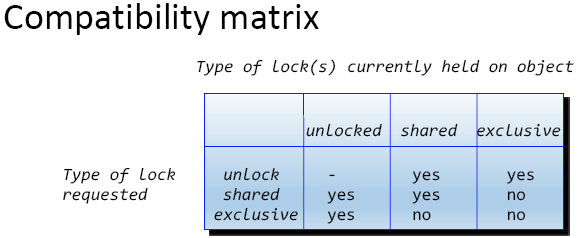
\includegraphics[width=250pt]{./images/Compatibility-matrix.png}
        \caption{\label{fig:Compatibility-matrix}Compatibility matrix}
    \end{figure}
    \item Lock manager implements locking protocol (set of rules to determine what locks can be granted in what situation (based on e.g. compatibility matrix ))
    \item Lock manager also uses a lock table (which locks are currently held by which transaction, which transactions are waiting to acquire certain locks, etc.)
    \item Lock manager needs to ensure ‘fairness’ of transaction scheduling to, e.g., avoid starvation        
\end{itemize}
\subsubsection{Two-Phase Locking Protocol (2PL)}
\begin{itemize}
    \item Before a transaction can read (update) a database object, it should acquire a shared (exclusive) lock on that object
    \item Lock manager determines if requested locks can be granted, based on compatibility matrix
    \item Acquiring and releasing locks occurs in 2 phases
    \begin{itemize}
        \item growth phase: locks can be acquired but no locks can be released
        \item shrink phase: locks are gradually released, and no additional locks can be acquired
    \end{itemize}
    \item Variants: Rigorous 2PL: transaction holds all its locks until it is committed \&\& Static 2PL (Conservative 2PL): transaction acquires all its locks right at the start of the transaction
    \item Two-Phase Locking Protocol \ref{fig:2PL}
    \item Lost update problem with locking \& Uncommitted dependency problem with locking
    \item Revisit the uncommitted dependency problem
    \begin{itemize}
        \item problem is resolved if T2 holds all its locks until it is rolled back
        \item with 2PL protocol, locks can already be released before the transaction commits or aborts (shrink phase)
    \end{itemize}
    \item Cascading Rollback should be applied recursively
    \item \textrightarrow best way to avoid this, is for all transactions to hold their locks until they have reached the ‘committed’ state (e.g., rigorous 2PL)
\end{itemize}
\begin{figure}
    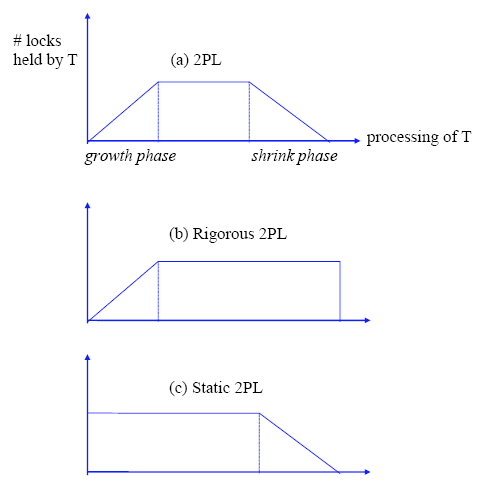
\includegraphics[width=300pt]{./images/2PL.png}
    \caption{\label{fig:2PL}Two-Phase Locking Protocol}
\end{figure}
\subsection{Dealing with Deadlocks}
\begin{itemize}
    \item A deadlock occurs if 2 or more transactions are waiting for one another’s’ locks to be released
    \item Deadlock prevention can be achieved by static 2PL (transaction must acquire all its locks upon the start)
    \item Detection and resolution
    \begin{itemize}
        \item wait for graph consisting of nodes representing active transactions and directed edges Ti  \textrightarrow Tj for each transaction Ti that is waiting to acquire a lock currently held by transaction Tj
        \item deadlock exists if the wait for graph contains a cycle
        \item victim selection
    \end{itemize}
\end{itemize}
\subsection{Isolation Levels}
\begin{itemize}
    \item Level of transaction isolation offered by 2PL may be too stringent
    \item Limited amount of interference may be acceptable for better throughput
    \item Long-term lock is granted and released according to a protocol, and is held for a longer time, until the transaction is committed
    \item A short-term lock is only held during the time interval needed to complete the associated operation
    \item \textrightarrow use of short-term locks violates rule 3 of the 2PL protocol \& can be used to improve throughput!
    \item \textbf{Read uncommitted}
    \item \textbf{Read committed}
    \item \textbf{Repeatable read}
    \item \textbf{Serializable}        
\end{itemize}
Isolation Levels \ref{fig:isolation-levels}
\begin{figure}
    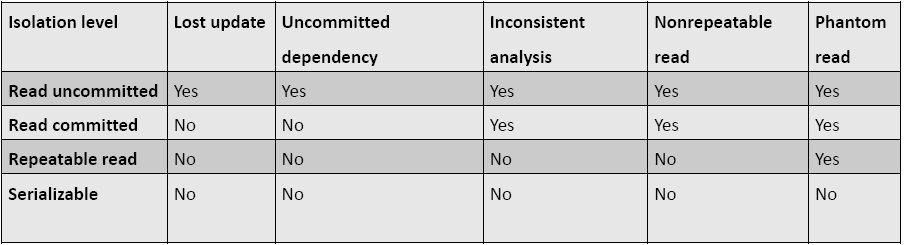
\includegraphics[width=\textwidth]{./images/isolation-levels.png}
    \caption{\label{fig:isolation-levels}Isolation Levels}
\end{figure}
\section{Lock Granularity}
\begin{itemize}
    \item Database object for locking can be a tuple, a column, a table, a tablespace, a disk block, etc.
    \item Trade-off between locking overhead and transaction throughput
    \item Many DBMSs provide the option to have the optimal granularity level determined by the database system
\end{itemize}
\section{ACID Properties of Transactions}
\begin{itemize}
    \item ACID stands for Atomicity, Consistency, Isolation and Durability
    \item \textbf{Atomicity} guarantees that multiple database operations that alter the database state can be treated as one indivisible unit of work
    \item \textbf{Consistency} refers to the fact that a transaction, if executed in isolation, renders the database from one consistent state into another consistent state
    \item \textbf{Isolation} denotes that, in situations where multiple transactions are executed concurrently, the outcome should be the same as if every transaction were executed in isolation
    \item \textbf{Durability} refers to the fact that the effects of a
    committed transaction should always be persisted into
    the database
\end{itemize}
\chapter{Datawarehousing \& Business Intelligence}
Knowledge piramid \ref{fig:knowledge-piramid}
\begin{figure}
    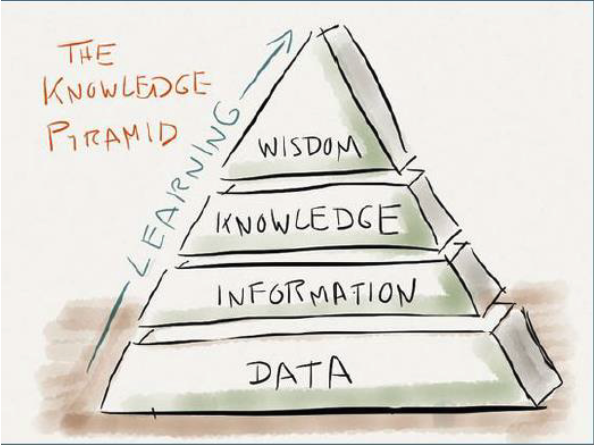
\includegraphics[width=250pt]{./images/knowledge-piramid.png}
    \caption{\label{fig:knowledge-piramid}Knowledge piramid}
\end{figure}
Business Intelligence (BI): Business intelligence, or BI, is a blanket term for technology that helps companies organize and query their data to help them improve operations and make more money.

Drivers for increasing use of BI: Digitalisation(ERP, CRM), Connectors between BI software and Business software, Data overflow, Complexity and Speed of change in the Business Environment, Reduce inefficiencies, inaccuracies, Decreasing Cost

Datawarehouse: A data warehouse is an integrated, subject oriented, time
variant and non volatile collection of data to support decisions
taken on management level.

\subsection{Properties:}
\begin{itemize}
    \item Subject oriented
    \item Integrated
    \item Time
    \item Non volatile
    \item Aggregated data
\end{itemize}

\subsection{Goals of DWH:}
\begin{itemize}
    \item Reporting
    \item Analysis of events in the past or actual events
    \item Predictions based on trend analysis
    \item Multidimensional reporting
    \item Empowerment of end user by offering simplified reporting tools (cf. SQL: only specialist can write SQL)
    \item Data mining
\end{itemize}

\section{Advantages}
\begin{itemize}
    \item High ROI (return on investment)
    \item Competitive advantage (Decision makers get access to data that was not available, unknown or unused before.)
    \item Increased productivity of corporate decision-makers
    \begin{itemize}
        \item Decision makers get one consistent view on the enterprise
        \item Decision makers can make more substantial, more accurate and more consistent analysis
    \end{itemize}
\end{itemize}

\section{Architecture}
DWH components \ref{fig:dwh-components}
\begin{figure}
    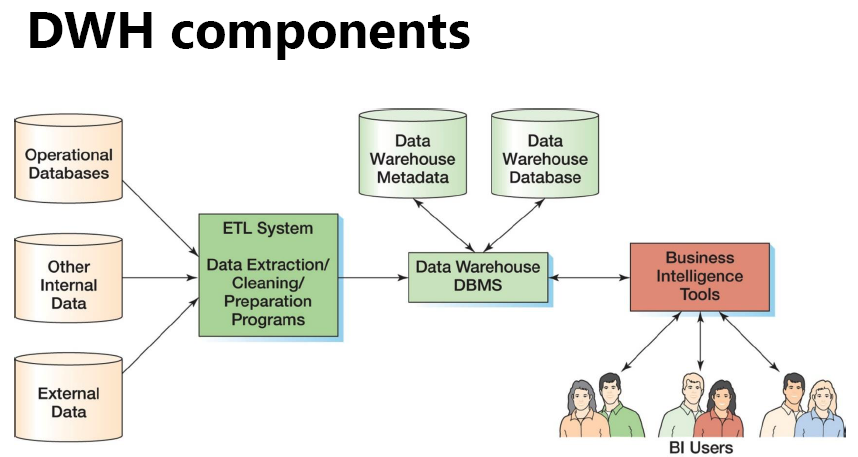
\includegraphics[width=250pt]{./images/dwh-components.png}
    \caption{\label{fig:dwh-components}DWH components}
\end{figure}
Read in slides

\section{Datamart}
A DB existing of a subset of company data to support the needs of a particular business unit for data analysis, or, to support users sharing the same needs for analyzing business processes.

Why a data mart?
\begin{itemize}
    \item To give users access to the data they analyse most frequently
    \item To offer data in a way that corresponds to the collective view of a group of users in a department or a group of users in the same business process
    \item To improve response time by offering lower data volumes
    \item To offer data in a format that fits the tools used by end users (OLAP, datamining tools)
    \item Reduction of complexity in the ETL process
    \item Reduction of cost as opposed to the setup of a complete DWH
\end{itemize}
\section{Data Mining Applications}
\begin{itemize}
    \item Perform what-if analyses
    \item Perform predictions ("predictive analysis")
    \item Facilitate the decision process
\end{itemize}
\section{Problems associated with DWH}
\begin{itemize}
    \item Underestimation of resources (costs) for ETL
    \item Hidden problems with source systems
    \item Required data not captured
    \item Increased end-user demands
    \item Data homogenization
    \item Need for concurrent support of several (historical) versions
    \item High demand for resources
    \item Data ownership
    \item High maintenance
    \item Long projects
    \item DWH creates expectation of user ‘empowering’: Make own reports, analyses
    \item Complexity of integration
    \item Complex change and version management
    \item \textrightarrow Night might be too short for ETL
\end{itemize}
\subsection{Problems with Operational data}
Dirty data, Missing values, Inconsistent data, Data not integrated, Wrong format, Too fine, Not fine enough, Too much data, Too many attributes, Too much volume

\section{Design}
\begin{itemize}
    \item Inmo
    \begin{itemize}
        \item Creation of a data model based on all data of the organisation
        \item Enterprise Data Warehouse (EDW)
        \item Used to distil data marts for each department
        \item Uses traditional methods for describing EDW
    \end{itemize}
    \item Kimball
    \begin{itemize}
        \item Starts by identifying the information requirements (referred to as analytical themes) and associated business processes of the enterprise \textrightarrow Data Warehouse Bus Matrix; 
    \end{itemize}
\end{itemize}

\subsection{Star schema}
A Star schema is a logical structure that 
has a fact table (containing factual data) in the center, surrounded by denormalized dimension tables containing reference data).
\begin{itemize}
    \item Fact table contains data about facts (E.g. factual data about sales of property: sales price, commission percentage)
    \item Dimension table contains reference informat (property data (address, etc), buyer, owner)
    \item Facts are generated by events that happened (e.g. a sale)
    \item Most probably facts never change
\end{itemize}
\subsection{Snowflake schema}
Snowflake schema is a variant of the star schema that has a fact table in the centre, surrounded by normalised dimension tables.

\subsection{Specific Schema Issues}
\begin{itemize}
    \item Surrogate keys
    \begin{itemize}
        \item StoreKey, ProductKey, ShipperKey \textrightarrow Meaningless integers
        \item Cannot use business keys since they usually have a business meaning
        \item Surrogate keys essentially buffer the data warehouse from the operational environment
        \item Business keys are usually bigger in size \& also often re-used over longer periods of time
    \end{itemize}
    \item Granularity of the fact table
    \begin{itemize}
        \item Level of detail of one row of the fact able
        \item Higher (lower) granularity implies more (fewer) rows
        \item Trade-off between level of detailed analysis and storage requirements
        \item example: One tuple of the fact table corresponds to one line on a purchase order
    \end{itemize}
\end{itemize}
\subsubsection{Factless Fact Tables}
\subsubsection{Optimizing the dimension tables}
Dimension tables should be heavily indexed to improve query execution time. average between 5 and 10 indexes. \textbf{time}: TimeKey, Date, DayOfWeek, DayOfMonth, DayOfYear

Junk Dimensions: Deal with low cardinality attribute types such as flags or indicators. Eg. On-line Purchase (Y/N), Payment (cash or credit-card), Discount (Y/N)

Outrigger tables: Store a set of attribute types of a dimension table which are highly correlated, low in cardinality and updated simultaneously.

Slowly Changing Dimensions \& Rapidly changing dimensions

\section{Advantages of the dimensional model}
\begin{itemize}
    \item Efficiency
    \item Ability to handle changing requirements
    \item The model can easily adapt to changing needs because each dimension is equivalent to the fact table
    \item Extensibility
    \item Ability to model common business situations
    \item Predictable query processing
\end{itemize}
    \section{Datawarehousing Delaware}
Analytics. Data, analaytics, human input, decision, action.
Met data kan je de kwaliteit van een proces verhogen. ERP maakt vb. veel data.

\begin{enumerate}
    \item Connect/verbind
    \begin{itemize}
        \item verbinden van ongelijksoortige data: DB, cloud, app, big data, NoSQL, XML ...
    \end{itemize}
    \item Combine/combineer
    \begin{itemize}
        \item Datawarehouse: voorbereiden data
        \item connect: nomaliseren views ongelijksoortige data
        \item combineer: ontdek, transformeer, bereid voor, verbeter, kwaliteit, integreer
        \item publish: deel, lever, beheers en werk samen.
    \end{itemize}
    \item Verwerk/gebruik in business applicaties
    \begin{itemize}
        \item Data verwerkers/gebruikers: enterprise, rapporteren, analyse, BI
    \end{itemize}
\end{enumerate}
\subsection{Voordelen datawarehouse}
\begin{itemize}
    \item Performantie
    \item betrouwbare data
\end{itemize}
Vb. van data \& DWH gebruiken: SAP groot touch screen live
Use Case:Ze hadden betrouwbare informatie nodig!
\begin{enumerate}
    \item Personal data
    \item Farm data
    \item Community data
\end{enumerate}


\end{document}

	

